\documentclass[reprint,english,notitlepage]{revtex4-1}  % 

\usepackage{silence}
\WarningFilter{revtex4-1}{Repair the float}

\usepackage[utf8]{inputenc}
\usepackage[english]{babel}
\usepackage{physics,amssymb} 
\usepackage{graphicx}        
\usepackage{xcolor}          
\usepackage{hyperref}        
\usepackage{tikz}             
\usepackage{listings} 
\usepackage{csquotes}
\usepackage{subfigure}  
\usepackage{here}
\usepackage{fontawesome}
\bibliographystyle{plain}
\hypersetup{ % this is just my personal choice, feel free to change things
    colorlinks,
    linkcolor={red!50!black},
    citecolor={blue!50!black},
    urlcolor={blue!80!black}}

%% Defines the style of the programming listing
%% This is actually my personal template, go ahead and change stuff if you want
\lstset{ %
	inputpath=,
	backgroundcolor=\color{white!88!black},
	basicstyle={\ttfamily\scriptsize},
	commentstyle=\color{magenta},
	language=Python,
	morekeywords={True,False},
	tabsize=4,
	stringstyle=\color{green!55!black},
	frame=single,
	keywordstyle=\color{blue},
	showstringspaces=false,
	columns=fullflexible,
	keepspaces=true}

%% TiKz stuff
\usetikzlibrary{positioning,chains}
\colorlet{myred}{red!80!black}
\colorlet{myblue}{blue!80!black}
\colorlet{mygreen}{green!60!black}
\colorlet{myorange}{orange!70!red!60!black}
\colorlet{mydarkred}{red!30!black}
\colorlet{mydarkblue}{blue!40!black}
\colorlet{mydarkgreen}{green!30!black}

\definecolor{mako1}{HTML}{38aaac}
\definecolor{mako2}{HTML}{357ba3}
\definecolor{mako3}{HTML}{40498e}


\begin{document}

%==========================================================
%------------------ Exercise content ----------------------
%==========================================================

%------------------ Title ---------------------------------
\title{Exercises week 38}
\author{Janita Ovidie Sandtrøen Willumsen \\ \faGithub \, \url{https://github.com/jovidie/FYS-STK4155}}        
\date{\today}
\noaffiliation

\maketitle

%------------------ Body -----------------------------------
% \mainmatter
\onecolumngrid
% %==========================================================
\section{Exercise 1}\label{sec:ex1}
%==========================================================
In Figure \ref{fig:ex1} I show that 
\begin{align*}
    \quad \frac{\partial (\mathbf{a}^{T}\mathbf{x})}{\partial \mathbf{x}} &= \mathbf{a}^{T} && \text{and} & \frac{\partial (\mathbf{a}^{T} \mathbf{A} \mathbf{a})}{\partial \mathbf{a}} &= \mathbf{a}^{T} (\mathbf{A} \mathbf{A}^{T}) && \text{and} & \frac{\partial (\mathbf{x} - \mathbf{A} \mathbf{s})^{T} (\mathbf{x} - \mathbf{A} \mathbf{s})}{\partial \mathbf{s}} &= -2 (\mathbf{x} - \mathbf{A} \mathbf{s})^{T} \mathbf{A}
\end{align*}

\begin{figure}
    \centering
    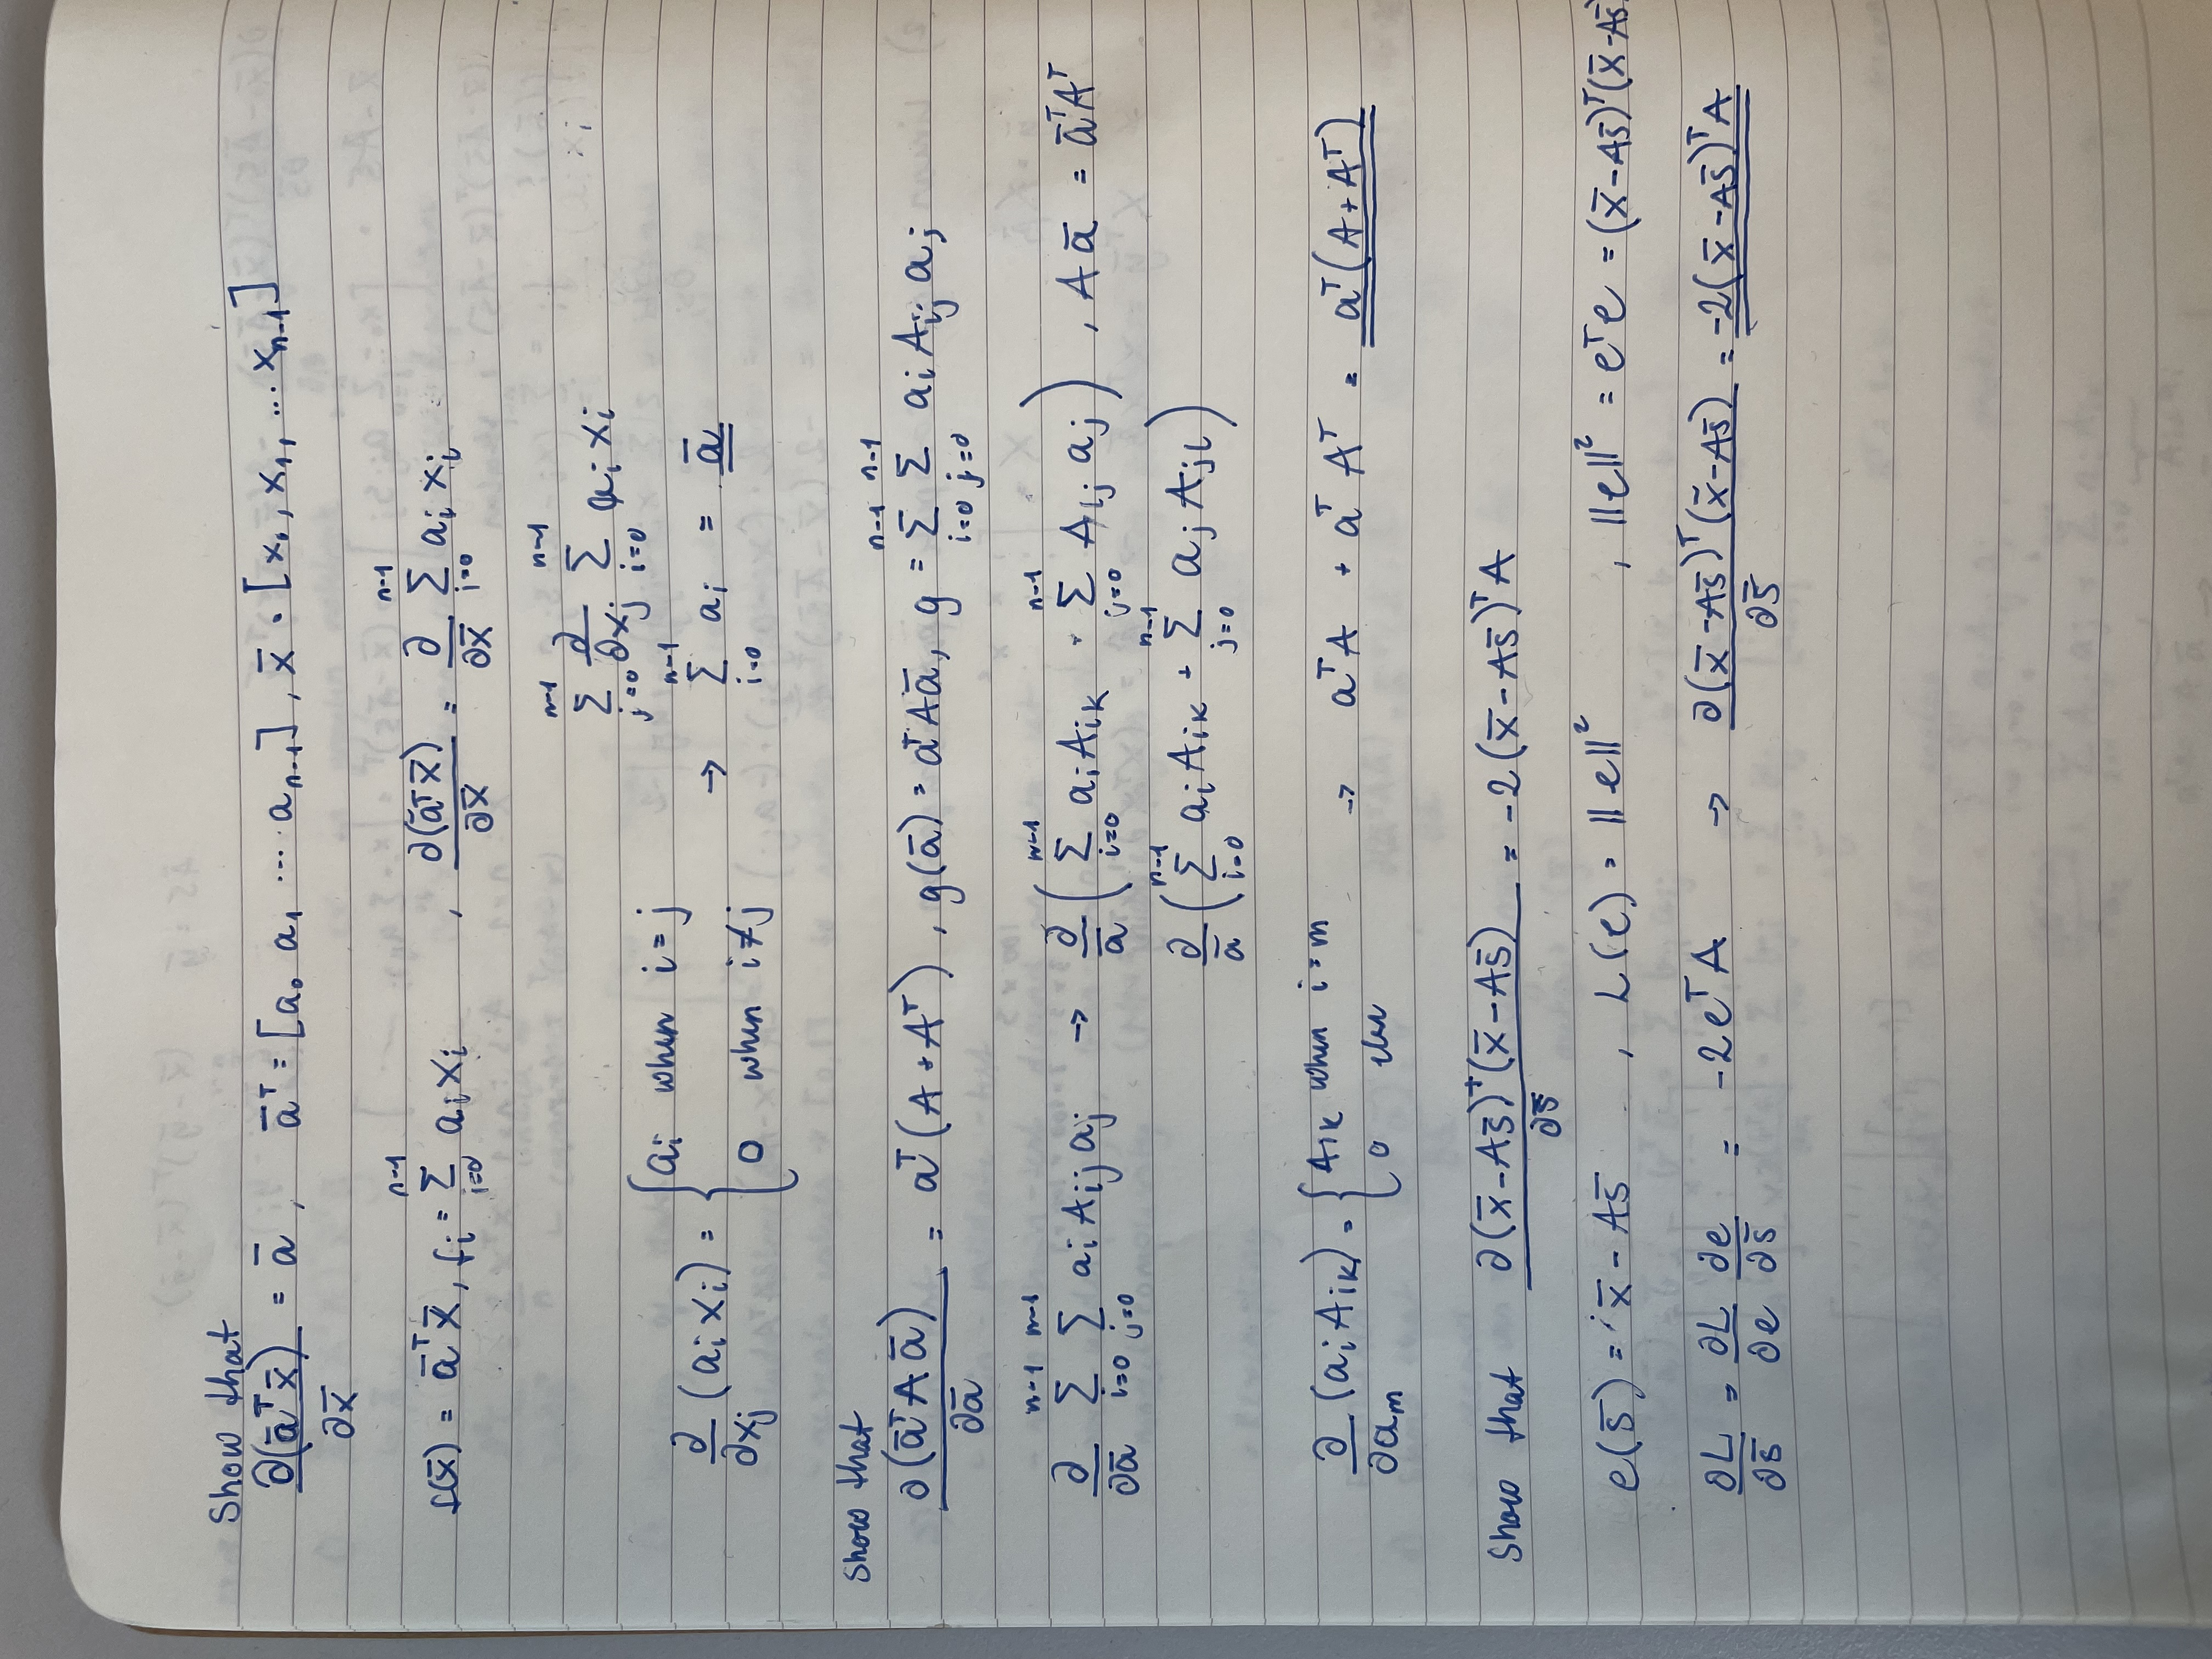
\includegraphics[width=0.8\linewidth, angle=270]{latex/figures/ex35-1.jpeg}
    \caption{Answer for exercise 1}
    \label{fig:ex1}
\end{figure}

\section{Exercise 2}\label{sec:ex2}
\begin{lstlisting}[language=Python]
import numpy as np
import matplotlib.pyplot as plt
from sklearn.linear_model import LinearRegression
from sklearn.preprocessing import PolynomialFeatures
from sklearn.metrics import mean_squared_error, r2_score

def exercise_35_2():
    x = np.random.rand(100)
    y = 2.0 + 5*x**2 + 0.1*np.random.randn(100)

    # Create design matrix 
    X = np.zeros((len(x), 3))
    X[:, 0] = 1
    X[:, 1] = x 
    X[:, 2] = x*x 

    beta = np.linalg.inv(X.T @ X) @ X.T @ y 
    y_pred = X @ beta

    poly = PolynomialFeatures(degree=2)
    X_model = poly.fit_transform(x[:, np.newaxis])
    model = LinearRegression()
    model.fit(X, y)
    model_pred = model.predict(X_model)

    mse_man = mean_squared_error(y, y_pred)
    r2_man = r2_score(y, y_pred)
    mse_sk = mean_squared_error(y, model_pred)
    r2_sk = r2_score(y, model_pred)
    
    fig, ax = plt.subplots()
    ax.plot(x, y, 'b.', label="Data")
    ax.plot(x, y_pred, 'ro', label=f"Own code: MSE = {mse_man:.4f}, R2 = {r2_man:.4f}")
    ax.plot(x, model_pred, 'gx', label=f"SciKit: MSE = {mse_sk:.4f}, R2 = {r2_sk:.4f}")
    ax.legend()
    plt.show()
\end{lstlisting}

\begin{figure}
    \centering
    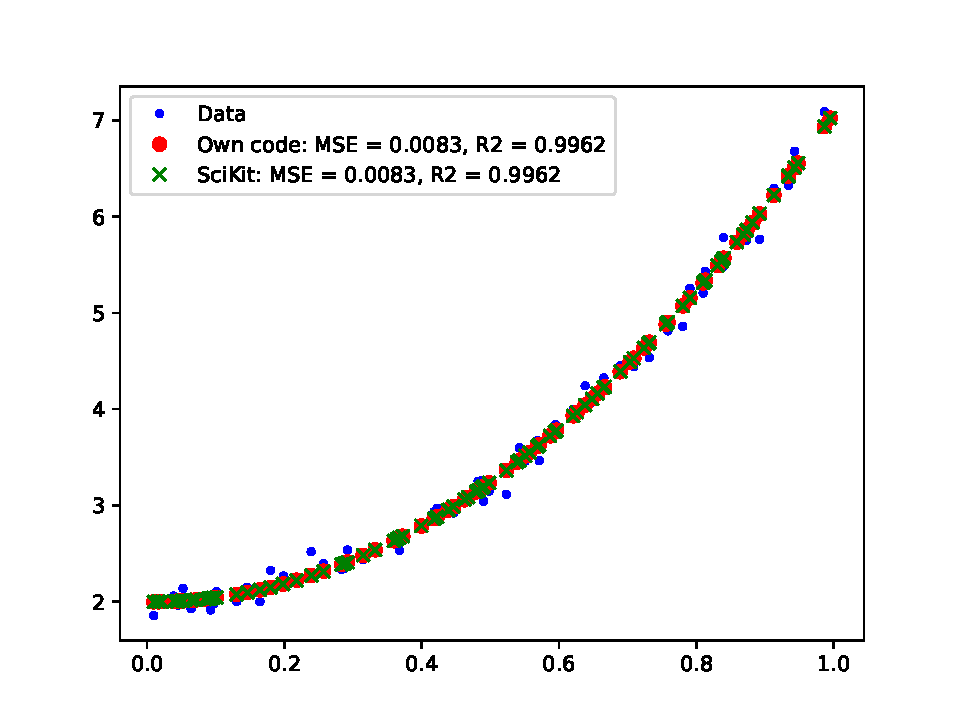
\includegraphics[width=0.5\linewidth]{latex/figures/week35_ex2.pdf}
    \caption{Results for exercise 2}
    \label{fig:ex2}
\end{figure}

\section{Exercise 3}\label{sec:ex3}
\begin{lstlisting}[language=Python]
class LinRegression:

    def __init__(self, degree) -> None:
        self._degree = degree + 1

    def _design_matrix(self, x):
        X = np.zeros((len(x), self._degree))
        X[:, 0] = 1
        for i in range(1, self._degree):
            X[:, i] = x**i
        return X

    def fit(self, x_train, y_train):
        self._X = self._design_matrix(x_train)
        self._X_T = self._X.T
        self._beta = np.linalg.inv(self._X_T @ self._X) @ self._X_T @ y_train 

    def predict(self, x_test):
        X_test = self._design_matrix(x_test)
        y_pred = X_test @ self._beta
        return y_pred 
    
    def compute_error(self, y_true, y_pred):
        self._mse = mse(y_true, y_pred)
        self._r2 = r2(y_true, y_pred)
        return self._mse, self._r2
        
def exercise_35_3():
    n = 100
    
    x = np.linspace(-3, 3, n)
    # x = x.reshape(-1, 1)
    noise = np.random.normal(0, 0.1, x.shape)
    y = np.exp(-x**2) + 1.5 * np.exp(-(x-2)**2) + noise 

    # poly = PolynomialFeatures(degree=4)
    # X = poly.fit_transform(x[:, np.newaxis])

    x_train, x_test, y_train, y_test = train_test_split(x, y, test_size=0.2)

    mse_history = []
    r2_history = []

    for degree in range(15):
        model = LinRegression(degree)
        model.fit(x_train, y_train)
        y_pred = model.predict(x_test)
        mse_loss, r2_val = model.compute_error(y_test, y_pred)
        mse_history.append(mse_loss)
        r2_history.append(r2_val)

    d = np.arange(15)
    fig, ax = plt.subplots()
    ax.plot(d, mse_history, label="MSE")
    ax.plot(d, r2_history, label="R2")
    ax.legend()
    plt.show()
    print(f"Optimal MSE = {mse_history[8]:.4f}, polynomial degree = {np.argmin(mse_history)}")
\end{lstlisting}

\begin{figure}
    \centering
    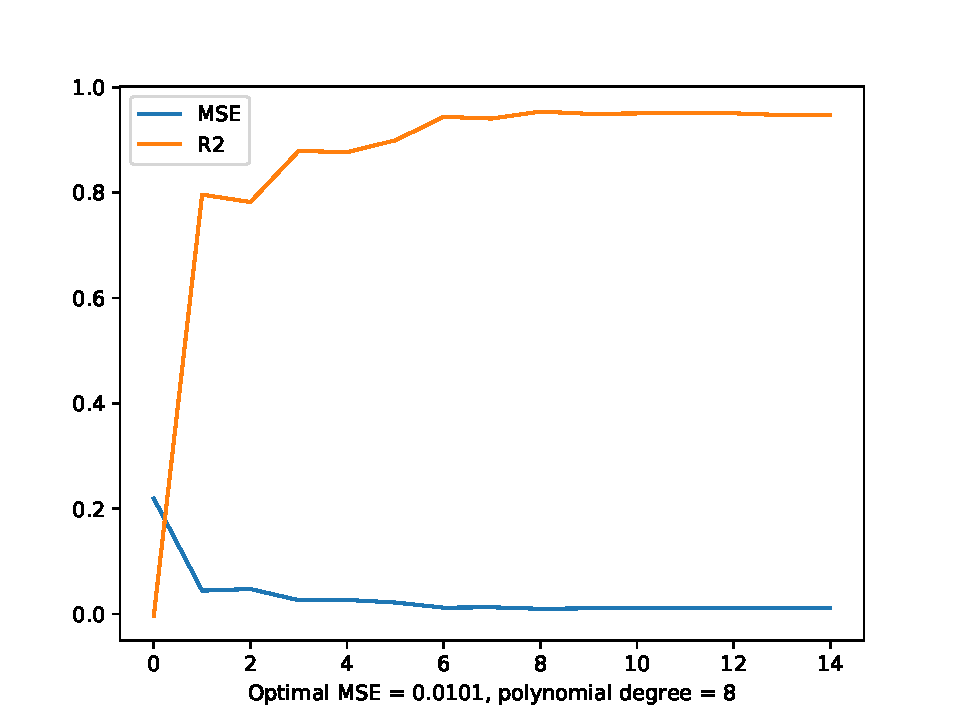
\includegraphics[width=0.5\linewidth]{latex/figures/week35_ex3.pdf}
    \caption{Results for exercise 3}
    \label{fig:ex3}
\end{figure}
% %==========================================================
\section{Exercise 1}\label{sec:ex1}
%==========================================================


%==========================================================
\section{Exercise 2}\label{sec:ex2}
%==========================================================


% %==========================================================
\section{Exercise 1}\label{sec:ex1}
%==========================================================
Assuming that $f(\mathbf{x})$ is a continuous function, and an error term $\mathbf{\epsilon} ~ N(0, \sigma^{2})$, we can approximate the function with the solution derived from a model $\mathbf{\tilde{y}} = X\mathbf{\beta}$. Which means the data can be described with $\boldsymbol{y} = X\mathbf{\beta} + \mathbf{\epsilon}$, giving the expectation value

\begin{align*}
    %\hskip\parindent
    \mathbb{E}(\mathbf{y}) &= \mathbb{E}(X\mathbf{\beta} + \mathbf{\epsilon}) \\
    &= \mathbb{E}(X\mathbf{\beta}) + \mathbb{E}(\mathbf{\epsilon}) && \text{where the expected value $\mathbf{\epsilon} = 0$} \\
    \mathbb{E}(y_{i}) &= \sum_{j=0}^{P-1} X_{i,j} \beta_{j} && \text{for the each element} \\
    &= X_{i,*} \beta && \text{where $_{*}$ replace the sum over index $j$} \\
\end{align*}

The variance for the element $y_{i}$ 
\begin{align*}
    \mathbb{V}(y_{i}) &= \mathbb{E} \big[ (y_{i} - \mathbb{E}(y_{i}))^{2} \big] \\
    &= \mathbb{E} ((X_{i,*} \beta_{i} + \epsilon_{i})^{2}) - (X_{i,*} \beta_{i})^{2} \\
    &= \mathbb{E} ((X_{i,*} \beta_{i})^{2}) + \mathbb{E} (2\epsilon_{i}X_{i,*} \beta_{i}) + \mathbb{E} (\epsilon^{2}) - (X_{i,*} \beta_{i})^{2} \\
    &= (X_{i,*} \beta_{i})^{2} + \mathbb{E} (\epsilon^{2}) - (X_{i,*} \beta_{i})^{2} \\
    &= \mathbb{E} (\epsilon^{2}) = \sigma^{2} \\
\end{align*}

With the OLS expression, the optimal parameter is
\begin{align*}
    \mathbf{\hat{\beta}} &= (\mathbf{X}^{T} \mathbf{X})^{-1} \mathbf{X}^{T} \mathbf{y} \\
\end{align*}

The expected value of $\mathbf{\hat{\beta}}$ is 
\begin{align*}
    \mathbb{E}(\mathbf{\hat{\beta}}) &= \mathbb{E}((\mathbf{X}^{T} \mathbf{X})^{-1} \mathbf{X}^{T} \mathbf{y}) \\
    &= (\mathbf{X}^{T} \mathbf{X})^{-1} \mathbf{X}^{T} \mathbb{E}(\mathbf{y}) && \text{using that $\mathbf{X}$ is a non-stochastic variable} \\
    &= (\mathbf{X}^{T} \mathbf{X})^{-1} \mathbf{X}^{T} \mathbf{X} \mathbf{\beta} && \text{using $\mathbb{E}(\mathbf{y}) = \mathbf{X} \mathbf{\beta}$} \\
    &= \mathbf{\beta} \\
\end{align*}

and the variance is 
\begin{align*}
    \mathbb{V}(\boldsymbol{\hat{\beta}}) &= \mathbb{E} \big[ (\boldsymbol{\hat{\beta}} - \mathbb{E}(\boldsymbol{\hat{\beta}}))^{2} \big] \\
    &= \mathbb{E} (((\boldsymbol{X}^{T} \boldsymbol{X})^{-1} \boldsymbol{X}^{T} \boldsymbol{y}) ((\boldsymbol{X}^{T} \boldsymbol{X})^{-1} \boldsymbol{X}^{T} \boldsymbol{y})^{T}) - \boldsymbol{\hat{\beta}}\boldsymbol{\hat{\beta}}^{T}  \\
    &= \mathbb{E} ((\boldsymbol{X}^{T} \boldsymbol{X})^{-1} \boldsymbol{X}^{T} \boldsymbol{y} \boldsymbol{y}^{T} \boldsymbol{X} (\boldsymbol{X}^{T} \boldsymbol{X})^{-1}) - \boldsymbol{\hat{\beta}}\boldsymbol{\hat{\beta}}^{T}  \\
    &= (\boldsymbol{X}^{T} \boldsymbol{X})^{-1} \boldsymbol{X}^{T} \mathbb{E} (\boldsymbol{y} \boldsymbol{y}^{T}) \boldsymbol{X} (\boldsymbol{X}^{T} \boldsymbol{X})^{-1} - \boldsymbol{\hat{\beta}}\boldsymbol{\hat{\beta}}^{T}  \\
    &= \boldsymbol{\beta} \boldsymbol{\beta}^{T} + \sigma^{2}((\boldsymbol{X}^{T} \boldsymbol{X})^{-1} \boldsymbol{X}^{T} \boldsymbol{X} (\boldsymbol{X}^{T} \boldsymbol{X})^{-1}) - \boldsymbol{\hat{\beta}}\boldsymbol{\hat{\beta}}^{T}  \\
    &= \sigma^{2}(\boldsymbol{X}^{T} \boldsymbol{X})^{-1} \\
\end{align*}


%==========================================================
\section{Exercise 2}\label{sec:ex2}
%==========================================================
Using the optimal $\mathbf{\hat{\beta}}^{Ridge}$, defined as 
\begin{align*}
    \boldsymbol{\hat{\beta}}^{Ridge} &= (\boldsymbol{X}^{T}\boldsymbol{X} + \lambda \boldsymbol{I})^{-1} \boldsymbol{X}^{T} \boldsymbol{y} \\
\end{align*}
The expectation value is then 
\begin{align*}
    \mathbb{E} (\mathbf{\hat{\beta}}^{Ridge}) &= \mathbb{E}((\mathbf{X}^{T}\mathbf{X} + \lambda \mathbf{I})^{-1} \mathbf{X}^{T} \mathbf{y}) \\
    &= (\mathbf{X}^{T}\mathbf{X} + \lambda \mathbf{I})^{-1} \mathbf{X}^{T} \mathbb{E}( \mathbf{y} ) && \text{since $\mathbf{X}$ and $\lambda \mathbf{I}$ are non-stochastic variables} \\
    &= (\mathbf{X}^{T}\mathbf{X} + \lambda \mathbf{I})^{-1} \mathbf{X}^{T} \mathbf{X} \mathbf{\beta} && \text{using $\mathbb{E} (\mathbf{y})$ from exercise 1} \\
\end{align*}
For $\lambda = 0$, $\mathbb{E} (\mathbf{\hat{\beta}}^{OLS})$. 

The variance 
\begin{align*}
    \mathbb{V}(\mathbf{\hat{\beta}}^{Ridge}) &= \mathbb{E} (\mathbf{\hat{\beta}}_{R} \mathbf{\hat{\beta}}_{R}^{T}) - (\mathbb{E} (\mathbf{\hat{\beta}}_{R}))^{2} \\
    &= \mathbb{E} (((\mathbf{X}^{T}\mathbf{X} + \lambda \mathbf{I})^{-1} \mathbf{X}^{T} \mathbf{y}) (((\mathbf{X}^{T}\mathbf{X} + \lambda \mathbf{I})^{-1} \mathbf{X}^{T} \mathbf{y}))^{T}) - (\mathbb{E} (\mathbf{\hat{\beta}}_{R}))^{2} \\
    &= (\mathbf{X}^{T}\mathbf{X} + \lambda \mathbf{I})^{-1} \mathbf{X}^{T} \mathbb{E} (\mathbf{y} \mathbf{y}^{T} ) \mathbf{X} ((\mathbf{X}^{T}\mathbf{X} + \lambda \mathbf{I})^{-1})^{T} - (\mathbb{E} (\mathbf{\hat{\beta}}_{R}))^{2} \\
    &= \sigma^{2}(\mathbf{X}^{T}\mathbf{X} + \lambda \mathbf{I})^{-1} \mathbf{X}^{T} \mathbf{X} ((\mathbf{X}^{T}\mathbf{X} + \lambda \mathbf{I})^{-1})^{T} \\
\end{align*}

Based on exercises solved and handed in previous semester \cite{willumsen:2023:projects}.
%==========================================================
\section{Exercise 1}\label{sec:ex1}
%==========================================================
The parameters $\mathbf{\beta}$ can be found by optimizing the cost function
\begin{equation*}
    C(\mathbf{X}, \mathbf{\beta}) = \frac{1}{n} \sum_{i=0}^{n-1} ( y_{i} - \Tilde{y}_{i} )^{2} = \mathbb{E} \big[ ( \mathbf{y} - \mathbf{\Tilde{y}} )^{2} \big] .
\end{equation*}

Assuming linearity, the expression can be written as 
\begin{equation*}
    \mathbb{E} \big[ ( \mathbf{y} - \mathbf{\Tilde{y}} )^{2} \big] = \mathbb{E} [ \mathbf{y}^{2} ] - 2 \mathbb{E} [ \mathbf{y} \mathbf{\Tilde{y}} ] + \mathbb{E} [ \mathbf{\Tilde{y}}^{2} ].
\end{equation*}

Looking at the first term
\begin{align*}
    \mathbb{E} [ \mathbf{y}^{2} ] &= \mathbb{E} [ ( f(\mathbf{x}) + \mathbf{\epsilon} )^{2} ] \\
    &= \mathbb{E} [ f(\mathbf{x})^{2} ] - 2 \mathbb{E} [ f(\mathbf{x}) \mathbf{\epsilon} ] + \mathbb{E} [ \mathbf{\epsilon}^{2} ] & \text{where $f(\mathbf{x})$ and $\epsilon$ are independent of $\mathbf{y}$, and eachother} \\
    &= f(\mathbf{x})^{2} + \sigma^{2} .
\end{align*}

The second term can be written as 
\begin{align*}
    \mathbb{E} [ \mathbf{y} \mathbf{\Tilde{y}} ] &= \mathbb{E} [ f(\mathbf{x} + \mathbf{\epsilon}) \mathbf{\Tilde{y}} ] \\
    &= \mathbb{E} [ f(\mathbf{x}) \mathbf{\Tilde{y}} ] + \mathbb{E} [ \epsilon \mathbf{\Tilde{y}} ] \\
    &=  f(\mathbf{x}) \mathbb{E} [ \mathbf{\Tilde{y}} ] & \text{since $\mathbb{E}[\mathbf{\epsilon}] = 0$} .
\end{align*}

The last term is the 2. moment, which can be written as 
\begin{align*}
    \mathbb{E} [ \mathbf{\Tilde{y}}^{2} ] &= \mathbb{V}[\mathbf{\Tilde{y}}] + (\mathbb{E} [ \mathbf{\Tilde{y}} ])^{2} 
\end{align*}

Combining all the terms, and rearranging gives us
\begin{align*}
    \mathbb{E} [ \mathbf{y}^{2} ] - 2 \mathbb{E} [ \mathbf{y} \mathbf{\Tilde{y}} ] + \mathbb{E} [ \mathbf{\Tilde{y}}^{2} ] &= f(\mathbf{x})^{2} + \sigma^{2} - 2 f(\mathbf{x}) \mathbb{E} [ \mathbf{\Tilde{y}} ] + \mathbb{V}[\mathbf{\Tilde{y}}] + (\mathbb{E} [ \mathbf{\Tilde{y}} ])^{2} 
    &= \mathbb{E} [ (\mathbf{y} - \mathbf{\Tilde{y}})^{2} ] + \mathbb{V}[\mathbf{\Tilde{y}}] + \sigma^{2} , 
\end{align*}
where 
\begin{align*}
    \mathbb{E} [ (\mathbf{y} - \mathbf{\Tilde{y}})^{2} ] = \text{Bias}[\mathbf{\Tilde{y}}]. 
\end{align*}

The bias-variance trade-off is a way to evaluate the how well the model is able to fit the test data. As seen in Figure \ref{fig:bias-variance}, when the polynomial degree is low, there is not much variance between the training data and the test data. However, the bias might be higher as it fails to predict the right complexity of the data. As the polynomial degree of the input increases, the variance increases. The bias decreases until the sufficient model complexity is reached. This is where the model is able to fit the training data, without overfitting, and also make good predictions on test data. 

\begin{figure}
    \centering
    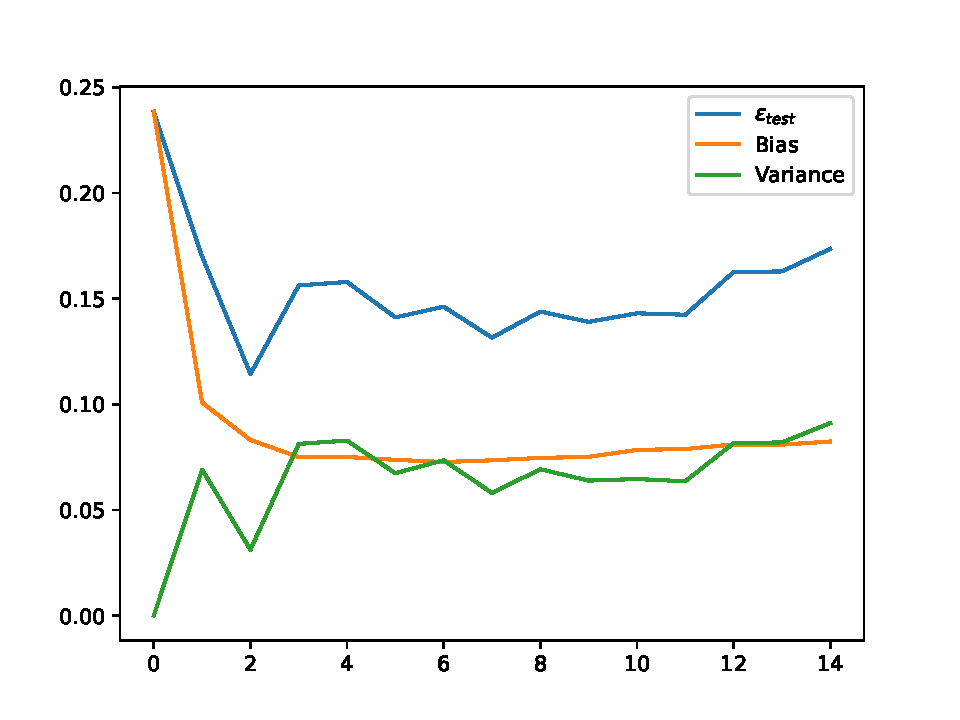
\includegraphics[width=0.5\linewidth]{latex/figures/ex38_noise.pdf}
    \caption{Bias-variance trade-off}
    \label{fig:bias-variance}
\end{figure}
% %==========================================================
\section{Abstract}\label{sec:ex1}
%==========================================================
In this project, I have studied three regression methods, Ordinary Least Squares (OLS), Ridge and Lasso, and compared their performance on synthetic and real terrain data. I found that the choice of method relies on the problem to be solved, and that the OLS method is sufficient when using noise free synthetic data from the Franke function. When introducing noise to the function, Ridge regression performed better as it did not overfit the data. I also performed a bias-variance trade-off analysis, using resampling methods such as bootstrap and cross-validation, and found the optimal polynomial degree for the input data.

%==========================================================
\section{Introduction}\label{sec:ex2}
%==========================================================
Artificial Intelligence (AI) and Machine Learning (ML) methods have many use cases, as it allows us to automate manual processes, make sense of complex data, and learn patterns not readily available. Today, the use of ML methods can be found in most industries, such as fraud detection, diagnosing disease, and increase efficiency in manufacturing processes \cite{forbes:2023:machine_learning}. 

In this project I will focus on Linear Regression ML methods, and their use in modeling and analysing terrain data. More specifically, I will study the difference in performance of Ordinary Least Squares, Ridge, and Lasso regression method, on synthetic terrain data generated using the Franke function. In addition, I will compare the model's performance when testing on real terrain data. To analyse the models in more detail, I will use resampling methods such as bootstrap and cross-validation, and study the bias-variance trade-off.

In Section II, I will present the methods and tools used in this project. Continuing with Section III, where I show the results and discuss my findings. In Section IV, I conclude and discuss possible future work.


% It is a growing field of vast potential. such as insurance and banking, 
% , which can be important in detecting changes in natural terrain
% \input{exercises/week40}
% \input{exercises/week41}
% \input{exercises/week42}
% \input{exercises/week43}
% \input{exercises/week44}
% \input{exercises/week45}
 
%------------------ Bibliography ---------------------------
% \newpage 
% \bibliographystyle{ksfh_nat}
\bibliography{references}


%==========================================================
%------------------ End of exercise content ---------------
%==========================================================

\end{document}
